\section{Literature Review}

\subsection{Computer-assisted Diagnosis and Management of Symptoms}

With the advent and distribution of personal computing devices, it became possible to diagnose and manage the symptoms of various diseases and disabilities. Unlike previous methods of manual, text-based symptom recordings, computer-based recordings are more easily manageable. Plus, with various computer-based interaction methods such as touch, sensors, and head-mounted displays (HMDs), the recording became more precise.

As such, previous studies have explored and proposed techniques that support diagnosis and management across various domains, such as developmental disabilities~\cite{shin2020talkingboogie}, overactive bladder~\cite{salai2019wee}, heart rate monitoring~\cite{li2019current}, and computer vision syndrome~\cite{liquideye}. By actively making use of computing devices, networks, and input methods, these studies revealed the possibility of computer-based diagnosis and management of various symptoms. Moreover, by utilizing highly mobile devices such as tablets and mobile phones, these works have lowered the barriers to diagnosis and health management.

\begin{figure*}[h!]
    \centering
    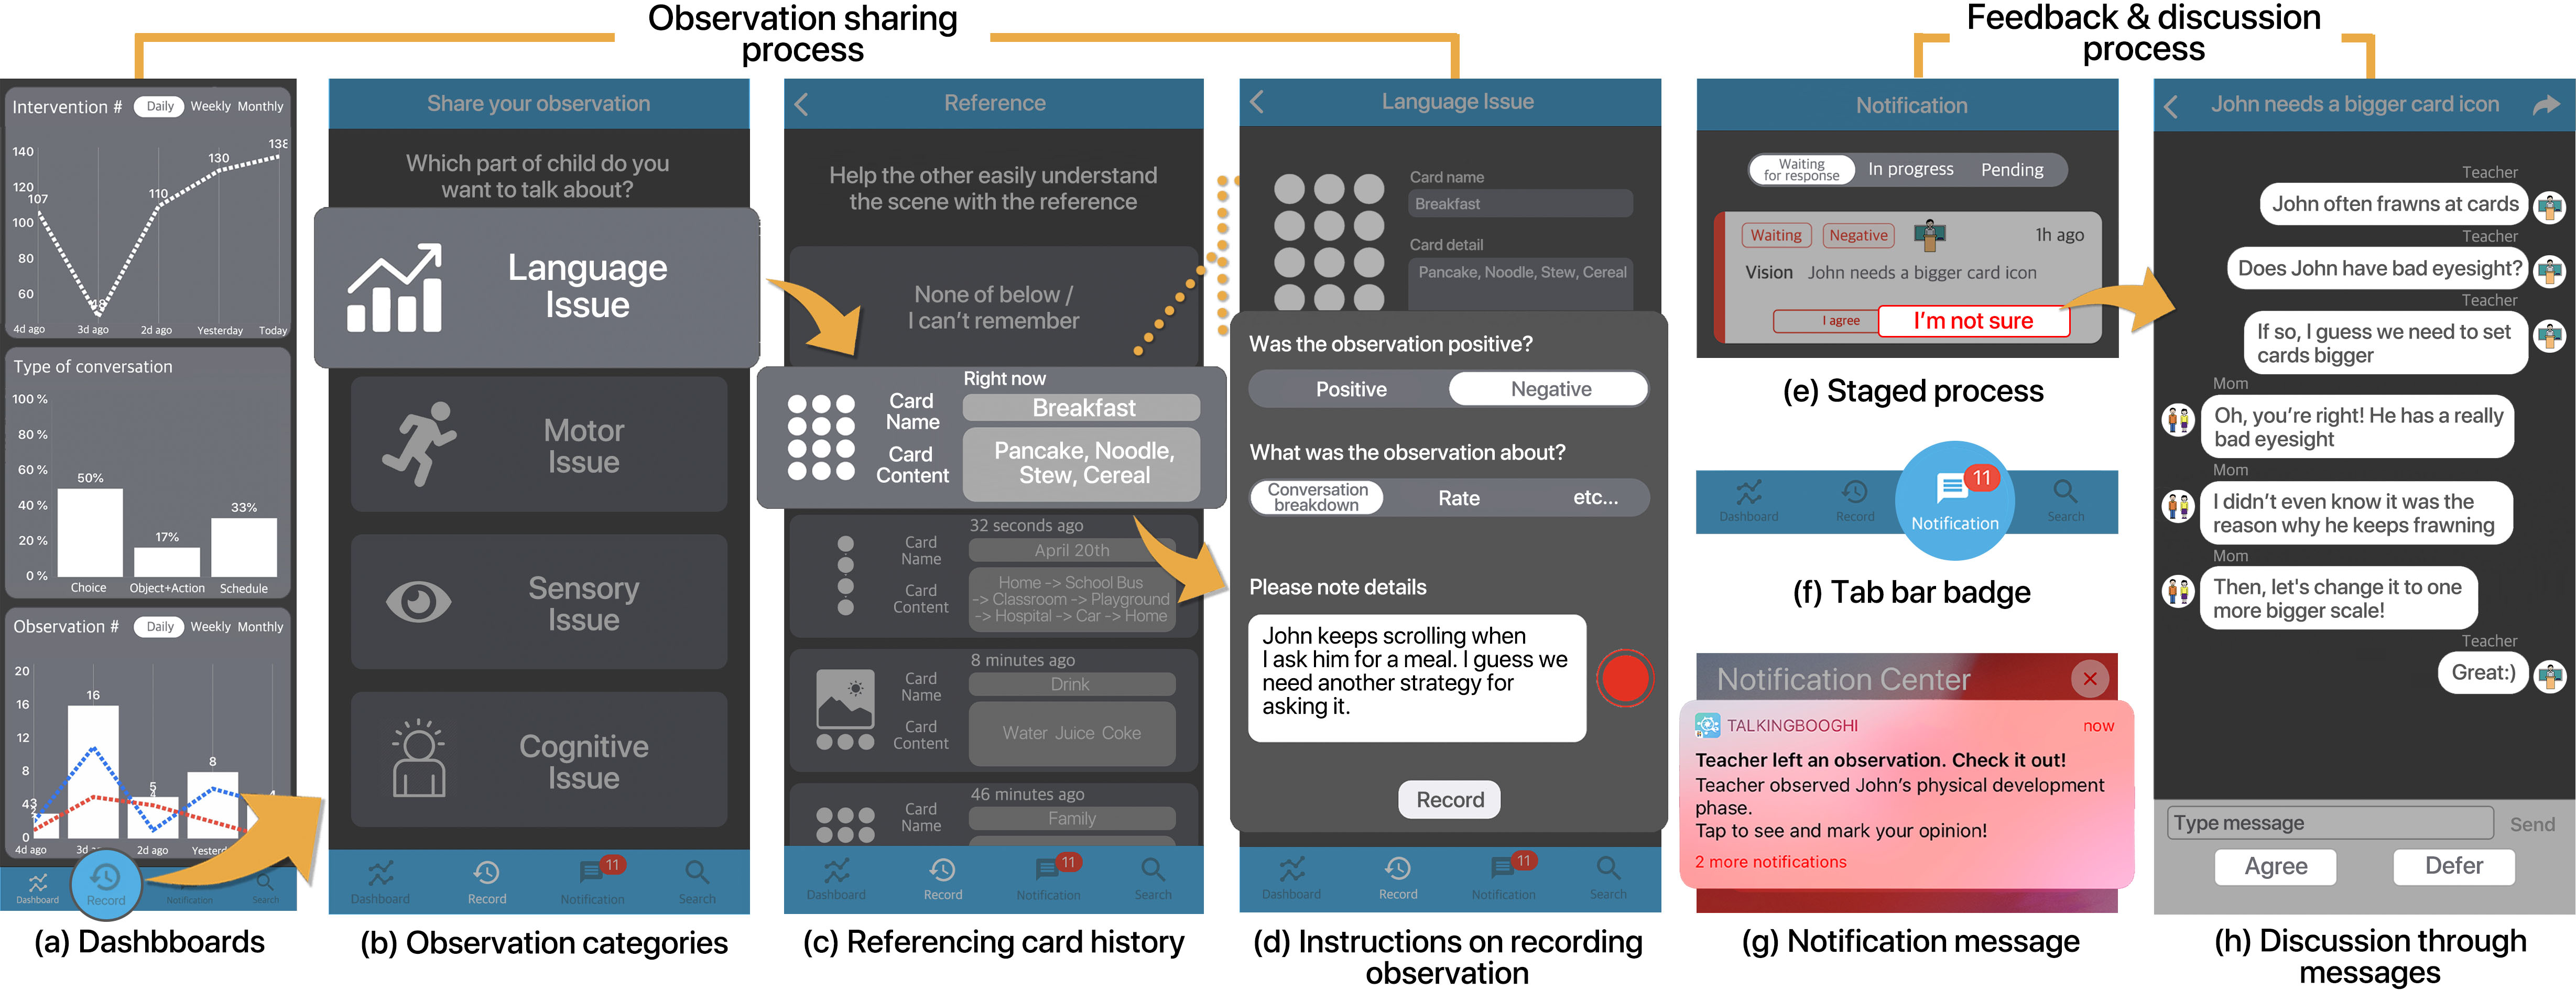
\includegraphics[width=\linewidth]{figure/tracker_explain_second.jpg}
    \caption{Example of computer-based application I designed for supporting parental monitoring of communicative issues for children with developmental disabilities~\cite{shin2020talkingboogie}}
    \label{fig:my_label}
\end{figure*}

Stemming from such design implications, I in this study seek for designing a mobile, self-reportable AMD application targeted to touch-based devices. Specifically, I considered that the web-based implementation of my feasible application might lower barriers to using the app, letting patients and practitioners utilize it regardless of device specifications, operating systems, and various constraints. As such, in this study, I propose a touch-based AMD diagnosing web app.

\subsection{Age-related Macular Degeneration (AMD) and Amsler Grid}

Age-related macular degeneration is a symptom that is accompanied by damage to the macula. According to Lim et al., AMD is a highly prevalent disease, with more than 20\% of aging populations affected by it~\cite{lim2012age}. Consisting of dry- and wet-AMD, AMD is often referred to as a disastrous disease due to its irreversible symptoms and leading patients to social isolation, it is important for patients to precisely understand the progress of the disease and manage it with an accurate diagnosis.

To diagnose AMD, Amsler grid (Figure~\ref{fig:amsler_grid}) has been widely used for the previous decades. Consisting of dozens of squares as a grid, Amsler grid aims to report distorted areas or blurred regions in sight verbally to the medical practitioners.

\begin{figure}[h!]
    \centering
    
\includegraphics[width=0.5\linewidth]{figure/amsler_grid.png}
    \caption{Amsler grid}
    \label{fig:amsler_grid}
\end{figure}

AMD is heterogeneous in terms of symptoms, with various visual issues often appearing altogether. Hence, it is important to precisely understand each symptom to design my tool user-centered and support patients with reporting each issue easily. Thus, by following the questionnaires of Schuchard's study for diagnosis using Amsler grid~\cite{schuchard1993validity}, I summarized the commonly reported symptoms of AMD that are observable through Amsler grid as follows:

\begin{itemize}
    \item \textbf{Distortion}: As illustrated in Figure~\ref{fig:symptoms}(b), the patients with AMD are known to often suffer from distortion of vision. Unlike Amsler grid viewed by people with normal sight (Figure~\ref{fig:symptoms}(a)), some of the lines are not shown parallel; the regions are irregular with its appearance either concave-shaped or convex-shaped.
    \item \textbf{Blurry sight}: Blurry sight is also a common symptom suffered by patients with AMD. This symptom is also described as dark spots, blurry region, or hole in the specific parts of sight.
    \item \textbf{Other symptoms}: Other symptoms include decreased visual acuity, less contrast, and slower adaptation of sight to the environment.
\end{itemize}

\begin{figure}[h!]
    \centering
    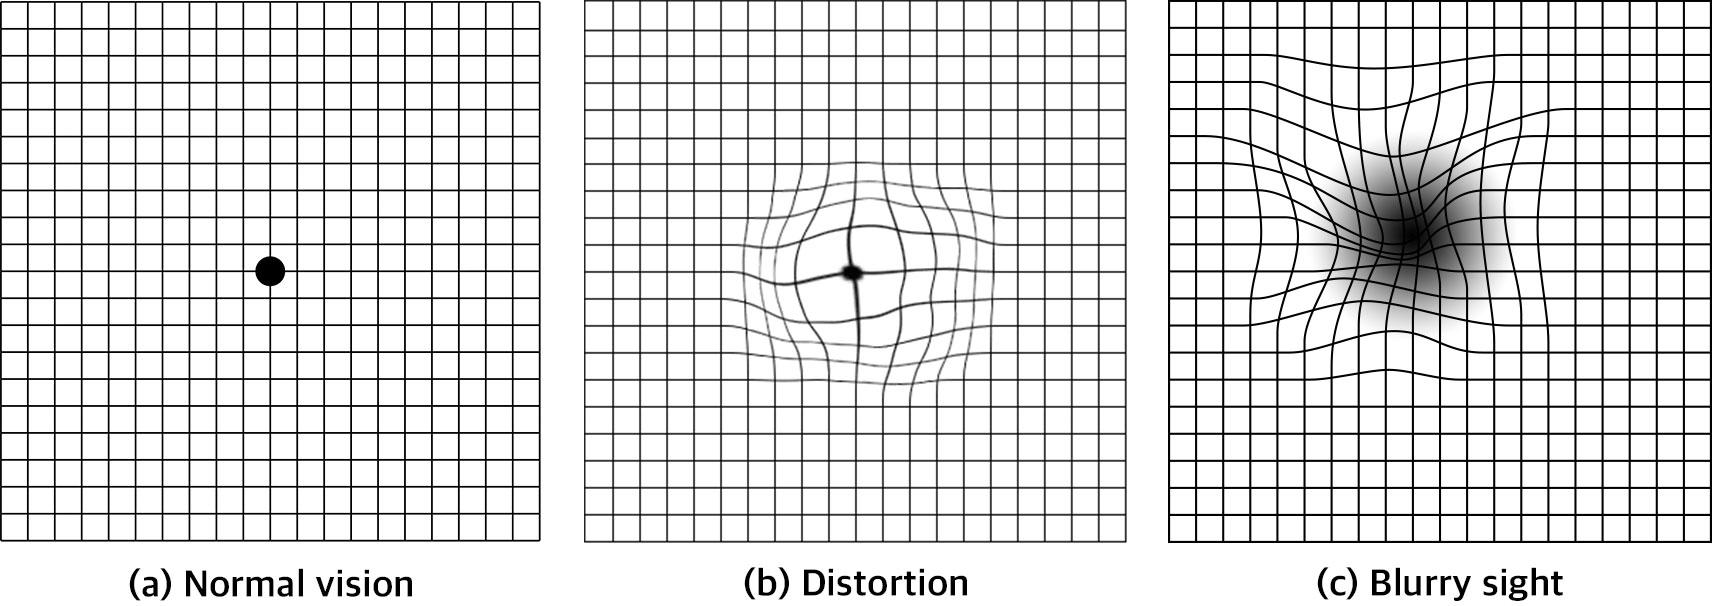
\includegraphics[width=\linewidth]{figure/symptoms.png}
    \caption{Common symptoms that are observable through Amsler grid testing}
    \label{fig:symptoms}
\end{figure}


\subsubsection{Diagnosis of AMD with Amsler grid}

While describing symptoms, there are important points that patients should adhere to, in terms of precise testing. I summarized some important guidelines that my possible design might also adhere to:

\begin{itemize}
    \item \textbf{Keeping a designated distance from the grid}: If the location of sight changes, the scope of vision also changes. Thus, the distance between grid and vision should be fixed for the precise report (e.g., 28 -- 30cm away for 10cm * 10cm grid)~\cite{elliott}.
    \item \textbf{Center-align the vision focus to the central point}: It is important for the patients to center-align their sight to the central point of the grid. The affected regions of vision are relative in location. In other words, the report might be affected by the focus of sight, thus requiring a person to fix the sight to the center~\cite{elliott}.
\end{itemize}

\subsection{Computer-based AMD Diagnosis}

Previous studies in the field of human-computer interaction, bioengineering, and health informatics have explored several techniques that support medical practitioners and patients to diagnose symptoms of AMD in computers. Noting that paper-based AMD testing had been shown unsuccessful in terms of precise diagnosis~\cite{fine1986earliest, roy1985vision}, these studies emphasized the feasibility of a computer-based approach for the precise and quantitative report of symptoms.

For example, Loewenstein et al. proposed MCPT, a system that supports patients to draw their region of symptoms on the computer~\cite{loewenstein2003replacing}. With basic input sources such as ordinary mouse and keyboard, these researchers sought to support a precise computer-based diagnosis. Mohaghegh and his colleagues developed a wearable system for diagnosing AMD symptoms~\cite{mohaghegh2016wearable}. They developed NGRID, a diagnosis system with a head-mounted device to support a more precise diagnosis of AMD. In addition to such approaches, the recent advent of 3D technologies made it possible to diagnose with 3D screens and glasses~\cite{kim2020novel}.

\begin{table}[htbp]
	\begin{center}
	\caption{Examples of AMD Diagnosis apps}
	\vspace{0.2cm}
	\begin{tabular}{|c|c|} \hline
		\textbf{Name} & \textbf{Description}\\ \hline
		\hline {\sc MCPT~\cite{loewenstein2003replacing}} & Drawing on the computer with ordinary mouse and keyboard\\
		\hline {\sc NGRID~\cite{mohaghegh2016wearable}} & Head-mounted Amsler-grid app\\
		\hline {\sc 3D Test~\cite{kim2020novel}} & Implemented with 3D screen and polarized glasses\\
		\hline
	\end{tabular}
	\label{tab1}
	\end{center}
\end{table}

As such, previous researchers were successful in exploring design spaces of novel diagnosis systems and proposing them. Yet, these approaches are limited in their efficiency and generalizability, since (i) they only made use of simple input devices that might not be sufficient in terms of accuracy or (ii) the techniques required costly devices that are not easily available. With the recent distribution of touch-based tablets, I found that these devices might give people a great opportunity to precisely note regions of the symptom without purchasing any costly device. Thus, in this study, I propose an AMD diagnosis app that lets users easily utilize it within their hand-held devices.